\chapter{Експериментальне дослідження чотирьохполюсників.} 
\label{chapter:first}

\section{Проба пера: дослідення перетворення прямокутних імпульсів}

Для отримання красивих картинок перетворення вхідного прямокутного сигналу очевидно був потрібний сам генератор сигналу. Оскільки розбиратися із версією, яка керується старичком ПК (який взагалі-то керується гордим Windows XP!) авторам було м'ягко кажучи лінь, було прийняте геніальне рішення - використати генератор DDS 9850, успішно апробований у \cite{lab3} та воскрешений у \cite{lab1}. Встановивши частоту $\omega = 10Hz$ та покрутивши трошки те, що крутити не треба було отримані красиві квадратні імпульси на вході та не менш красиві перетворені сигнали на виході \ref{fig:square}.

\begin{figure}[h]
	\begin{minipage}[h]{0.47\linewidth}
		\center{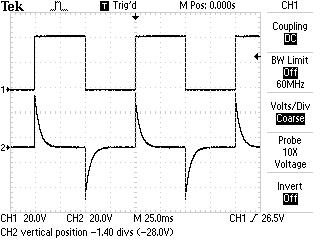
\includegraphics[width=1\linewidth]{square/D.png}} \\
	\end{minipage}
	\hfill
	\begin{minipage}[h]{0.47\linewidth}
		\center{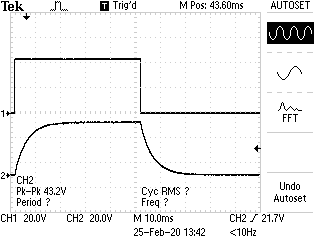
\includegraphics[width=1\linewidth]{square/I.png}} \\
	\end{minipage}
	\caption{Перетворення квадратних імпульсів для диферинціюючого та інтегруючого чотирьохполюсника}
	\label{fig:square}
\end{figure}

\section{Дослідження амплітудно-частотних та фазо-частотних характеристик приборів.}

Для виконання цього завдання ми подавали сигнал синусоїдальної форми різної частоти на вхід, та порівнювали з ним сигнал, що отримувався на виході з осцилографа. Здобуті надважким шляхом два набора точок у формі синусоїд \ref{fig:expsin} апроксимовувалися у програмі cern Root \cite{root}, а чисельні значення амплітуд та зсуву фаз порівнювалися, та записувалися відповідні значення $K(\omega)$ та $\phi(\omega)$. 

\begin{figure}[h]
	\center{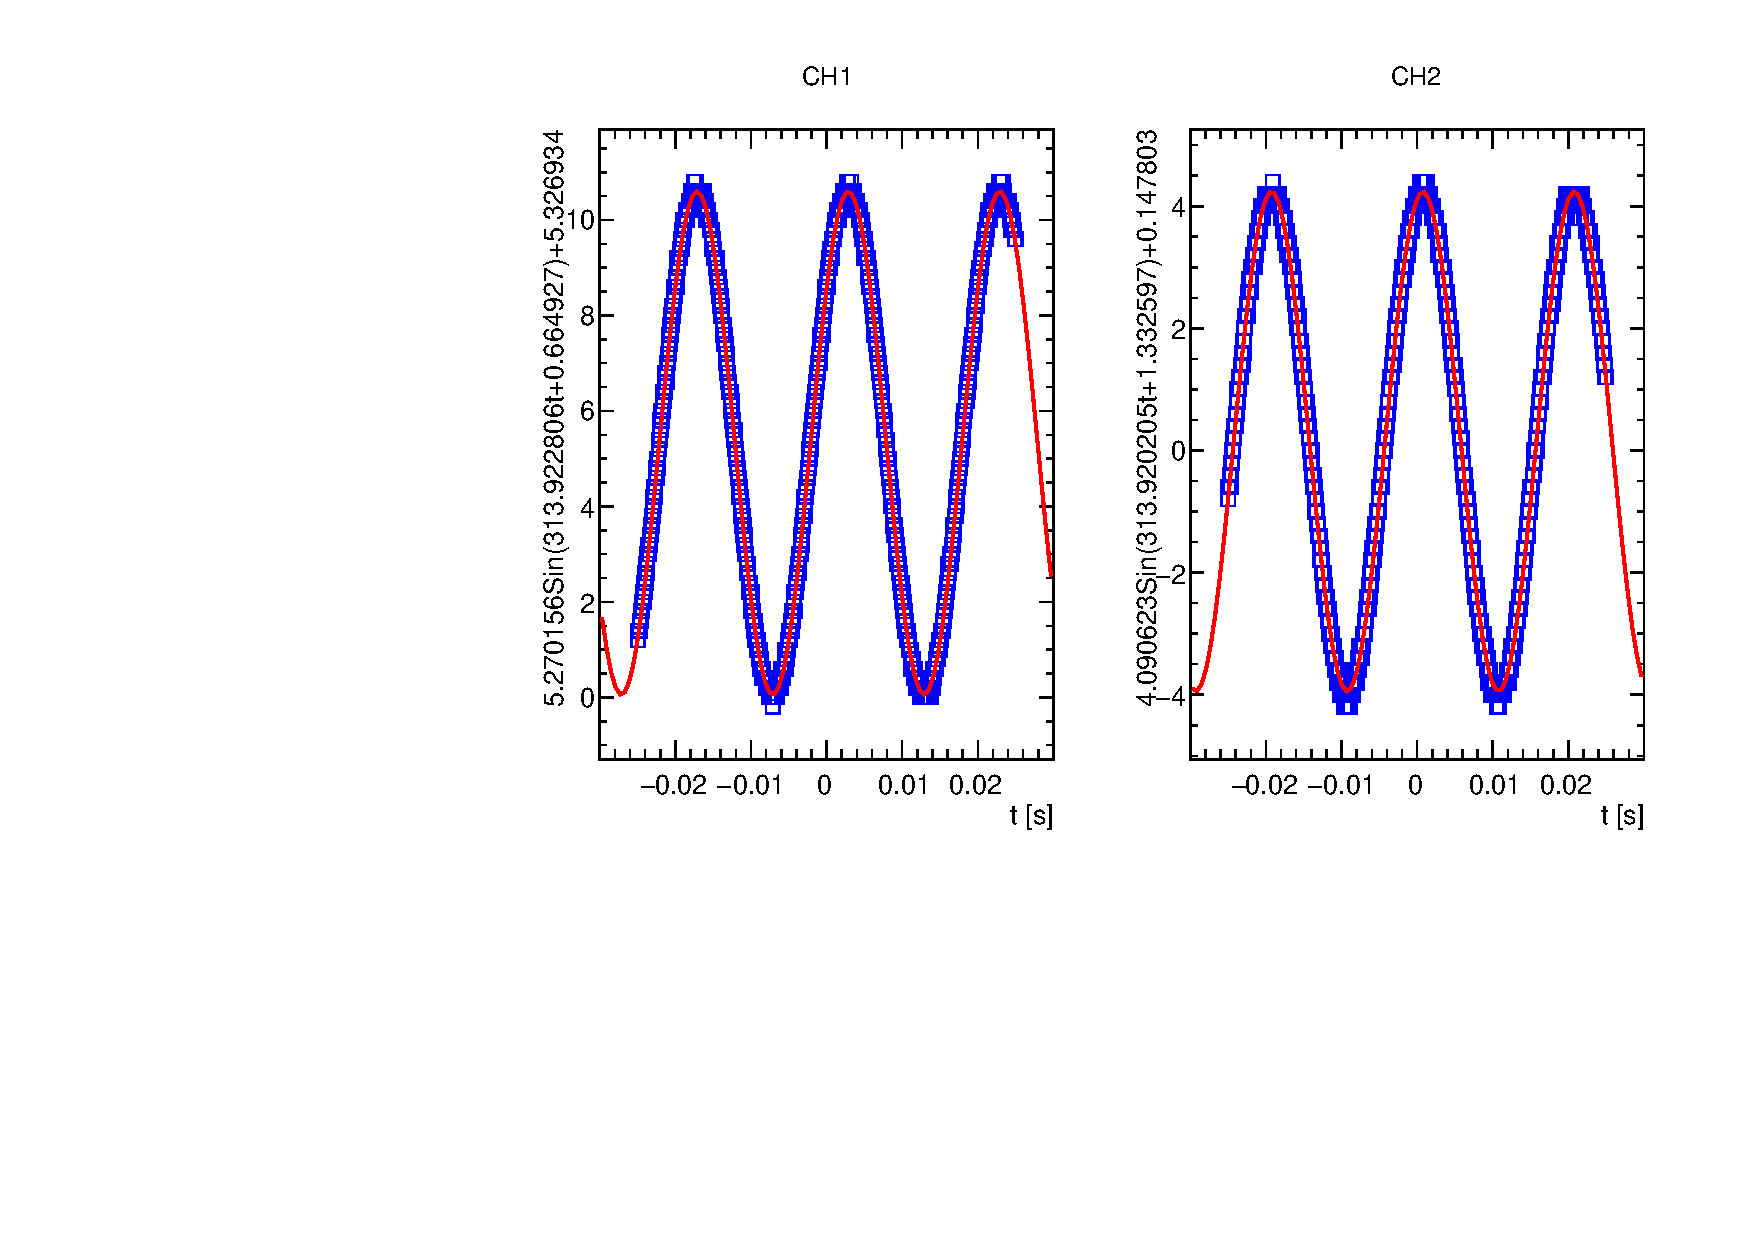
\includegraphics[width=1\linewidth,height=0.45\linewidth]{sind/sin.pdf}} \\
	\caption{Сигнал на вході (канал 1) та виході (канал 2) диферинціюйочого чотирьохполюсника при $\omega = 50Hz$. Параметри апроксимації написані у підписі до вертикальної осі.}
	\label{fig:expsinD}
\end{figure}

\begin{figure}[h]
	\center{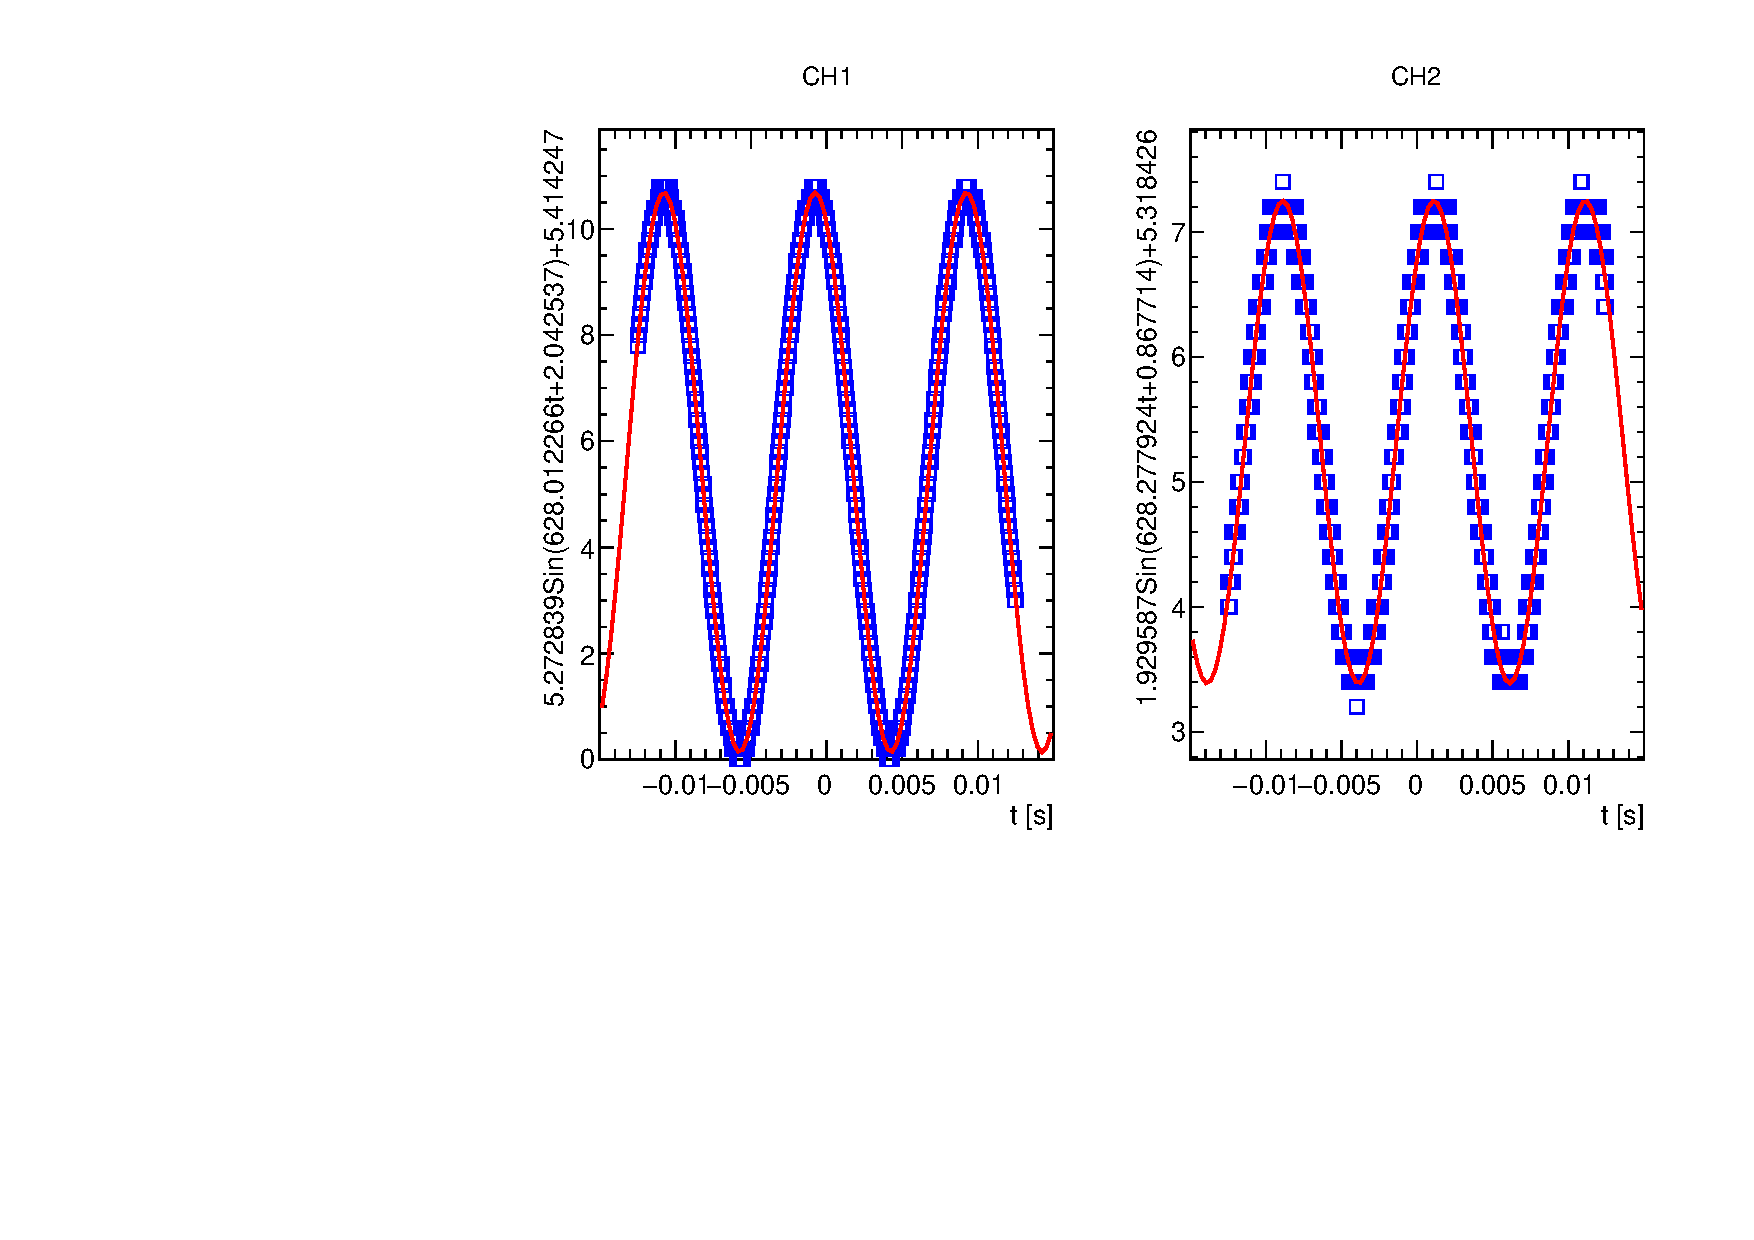
\includegraphics[width=1\linewidth,height=0.45\linewidth]{sini/sin.pdf}} \\
	\caption{Сигнал на вході (канал 1) та виході (канал 2) інтегруючого чотирьохполюсника при $\omega = 50Hz$. Параметри апроксимації написані у підписі до вертикальної осі.}
	\label{fig:expsinI}
\end{figure}

І таким чином ми отримували красиві графіки \ref{fig:expkph}. Звісно ми спробували апроксимувати ці точки за допомогою загальноприйнятих моделей \ref{theoryD} та \ref{theoryI} для диферинціюючих та інтегруючих чотирьохполюсників відповідно. 

\begin{equation}
	\begin{aligned}
		K = \frac{\omega RC}{\sqrt{1+(\omega R C)^2}}\\
		\phi = arctg(\frac{1}{\omega RC})
	\end{aligned}
	\label{theoryD}
\end{equation}

\begin{equation}
	\begin{aligned}
		K = \frac{1}{\sqrt{1+(\omega R C)^2}}\\
		\phi = -arctg(\omega RC)
	\end{aligned}
	\label{theoryI}
\end{equation}

Невідомим параметром при такій апроксимації виступає наглий добуток $RC$. Отримане значення (звісно за допомогою алгоритму MIGRAD/MINUIT) складало $RC = 0.0252943 \pm  0.000240748 s$. 
Якщо тепер порахувати теоретичне значення даної величини ($R = 200k\Omega$, $C = 154nF$) отримаємо значення $RC = 0.0308 s$ - \textbf{от що робить паразитний опір та ємність з хорошими \sout{людьми} чотирьохполюсниками.}

\begin{figure}[h]
	\begin{minipage}[h]{0.47\linewidth}
		\center{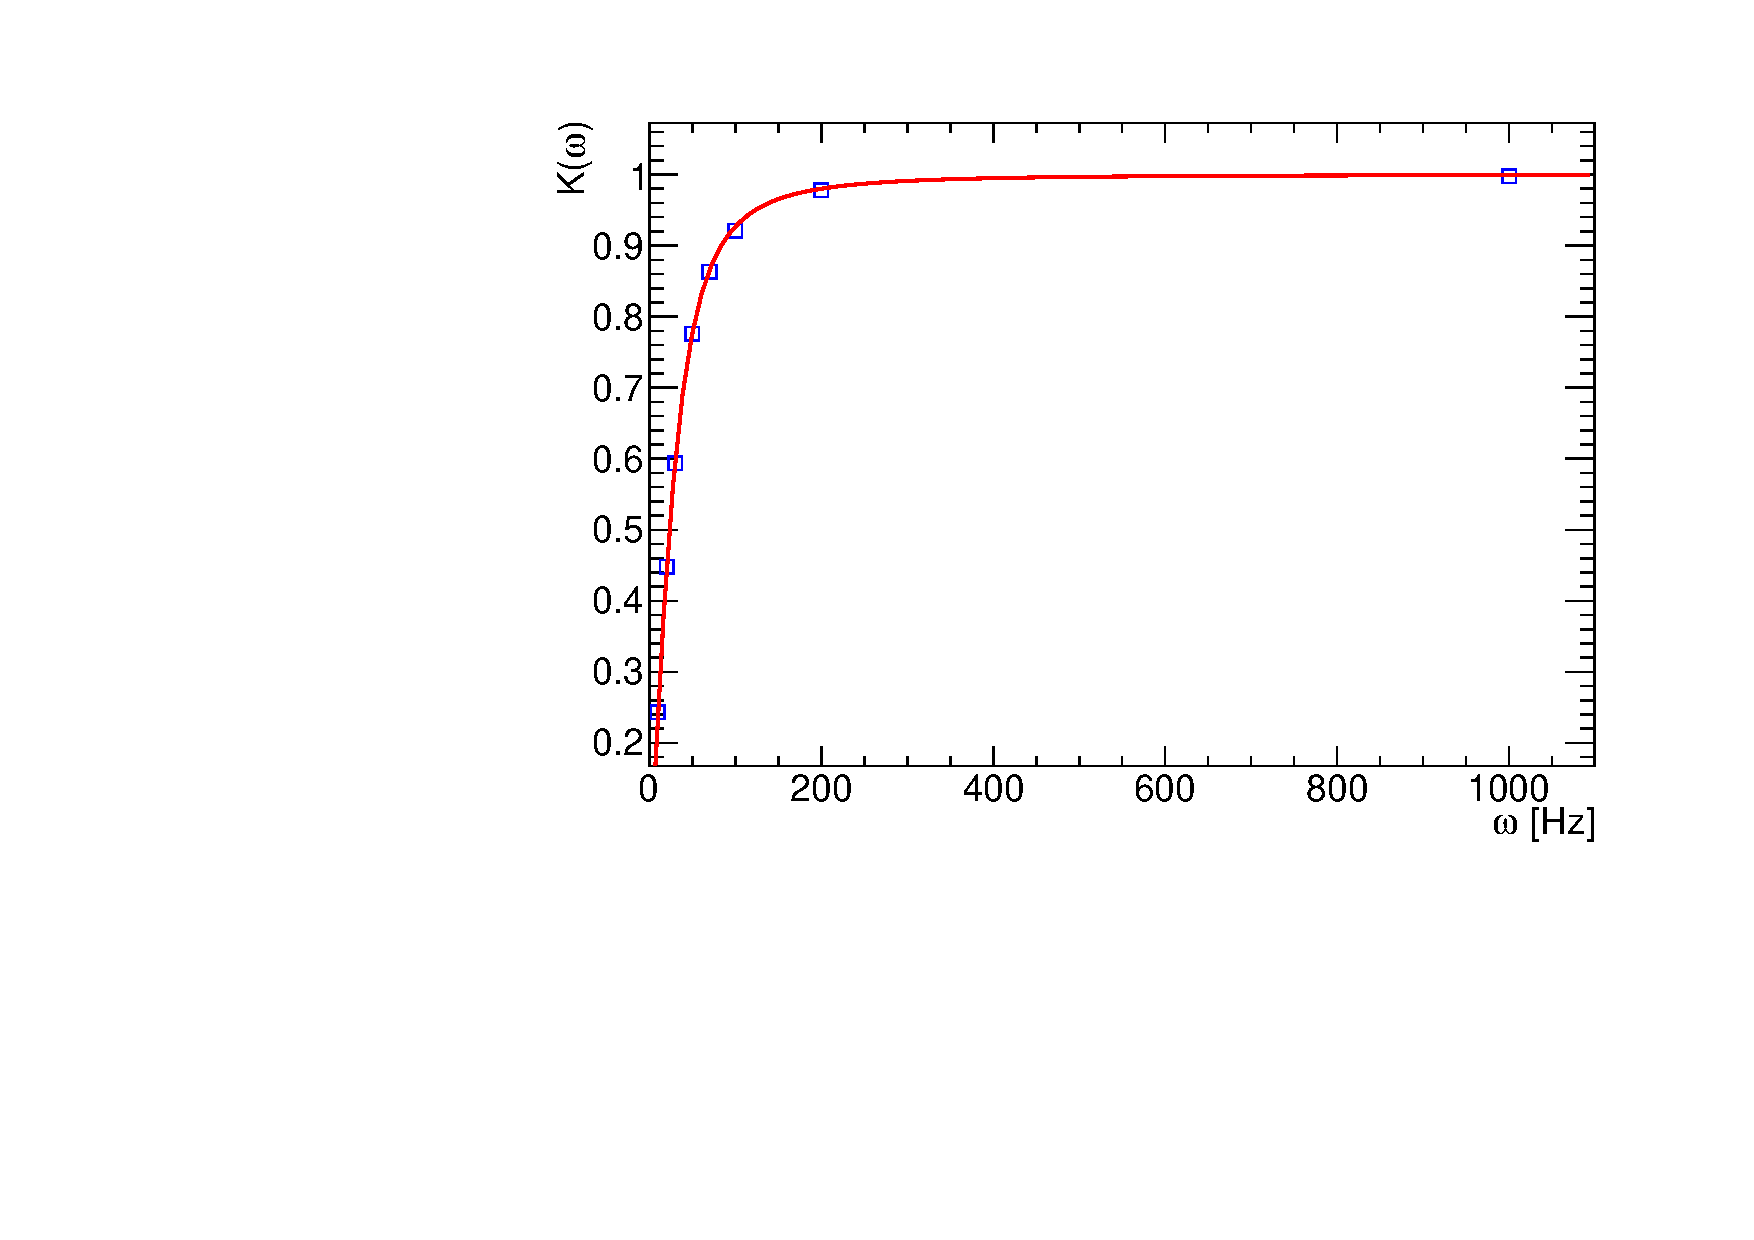
\includegraphics[width=1\linewidth]{sind/k.pdf}} \\$K(\omega)$ для диферинціюйочого чотирьохполюсника
	\end{minipage}
	\hfill
	\begin{minipage}[h]{0.47\linewidth}
		\center{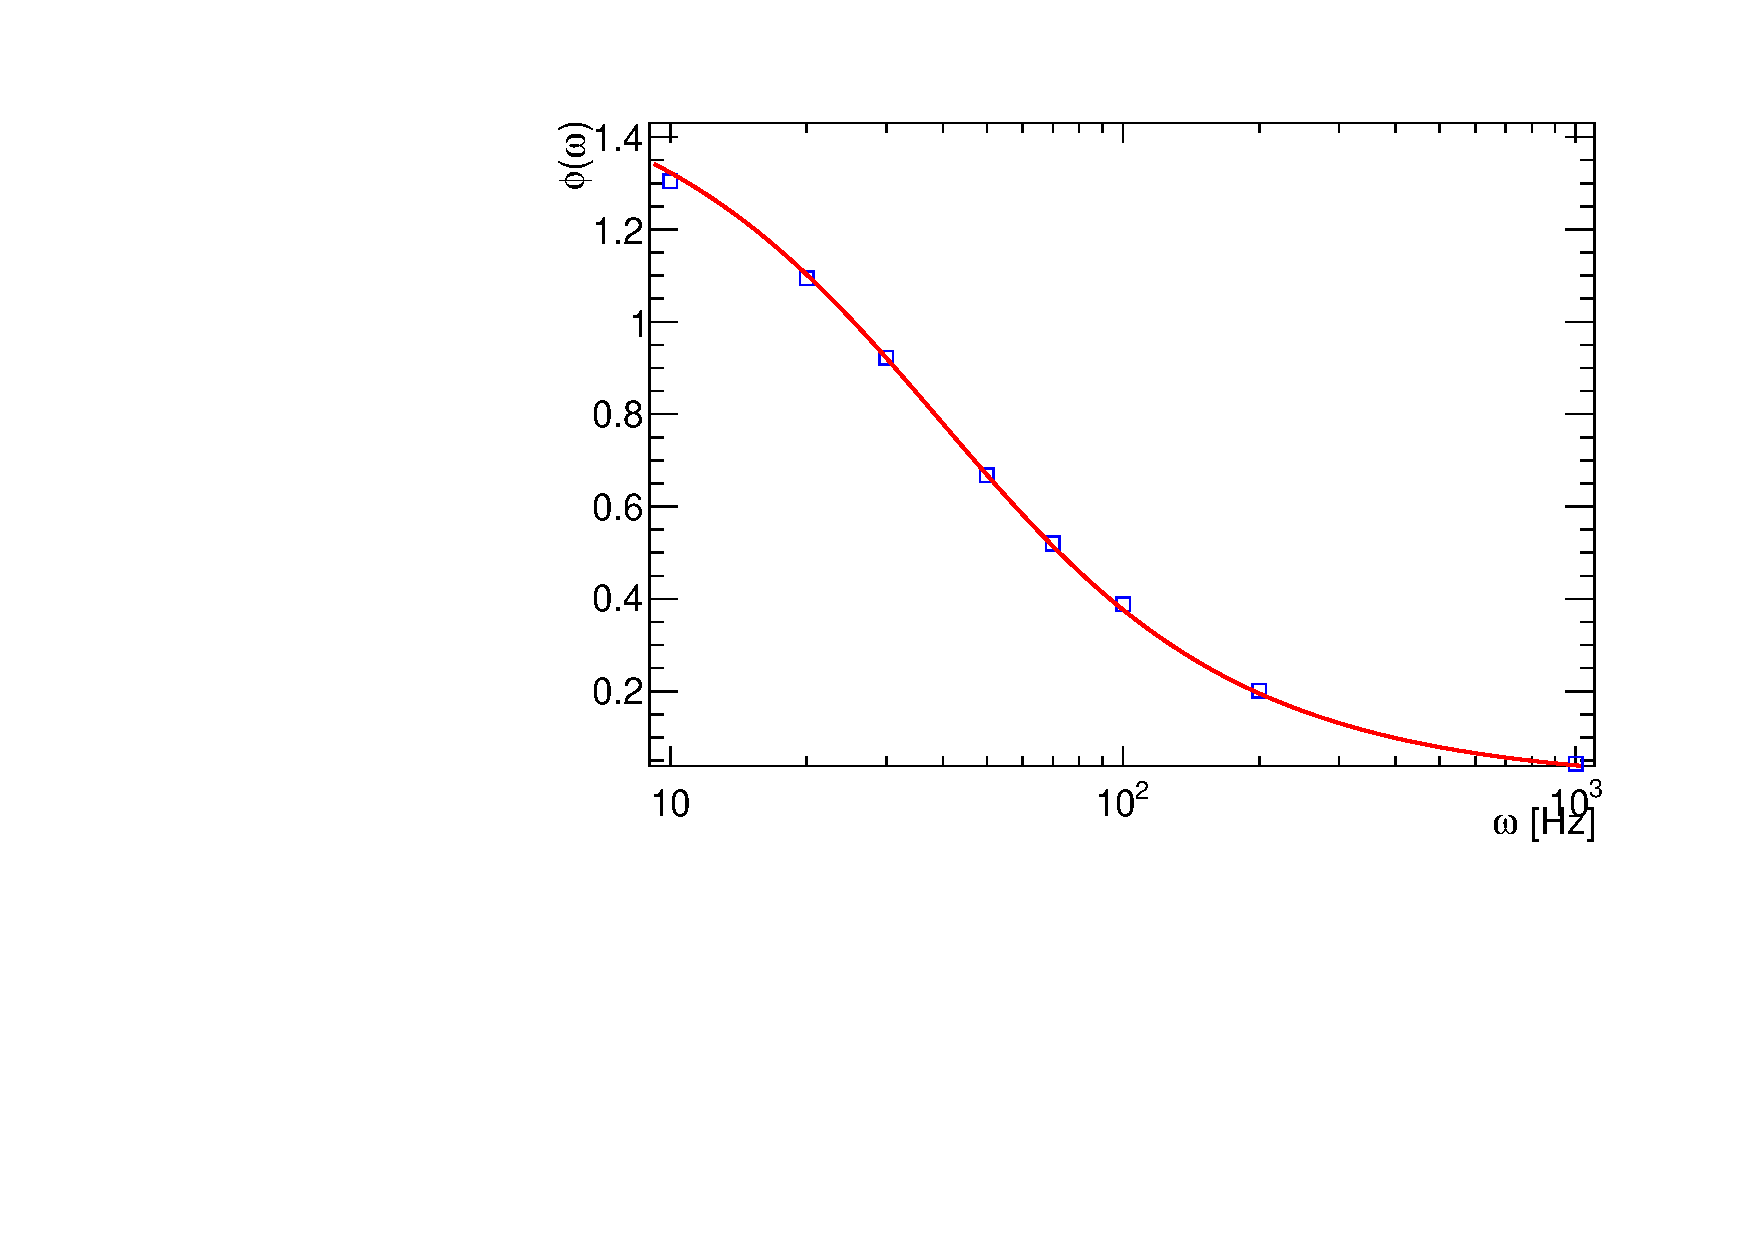
\includegraphics[width=1\linewidth]{sind/phi.pdf}} \\$\phi(\omega)$ для диферинціюйочого чотирьохполюсника
	\end{minipage}
	\vfill
	\begin{minipage}[h]{0.47\linewidth}
		\center{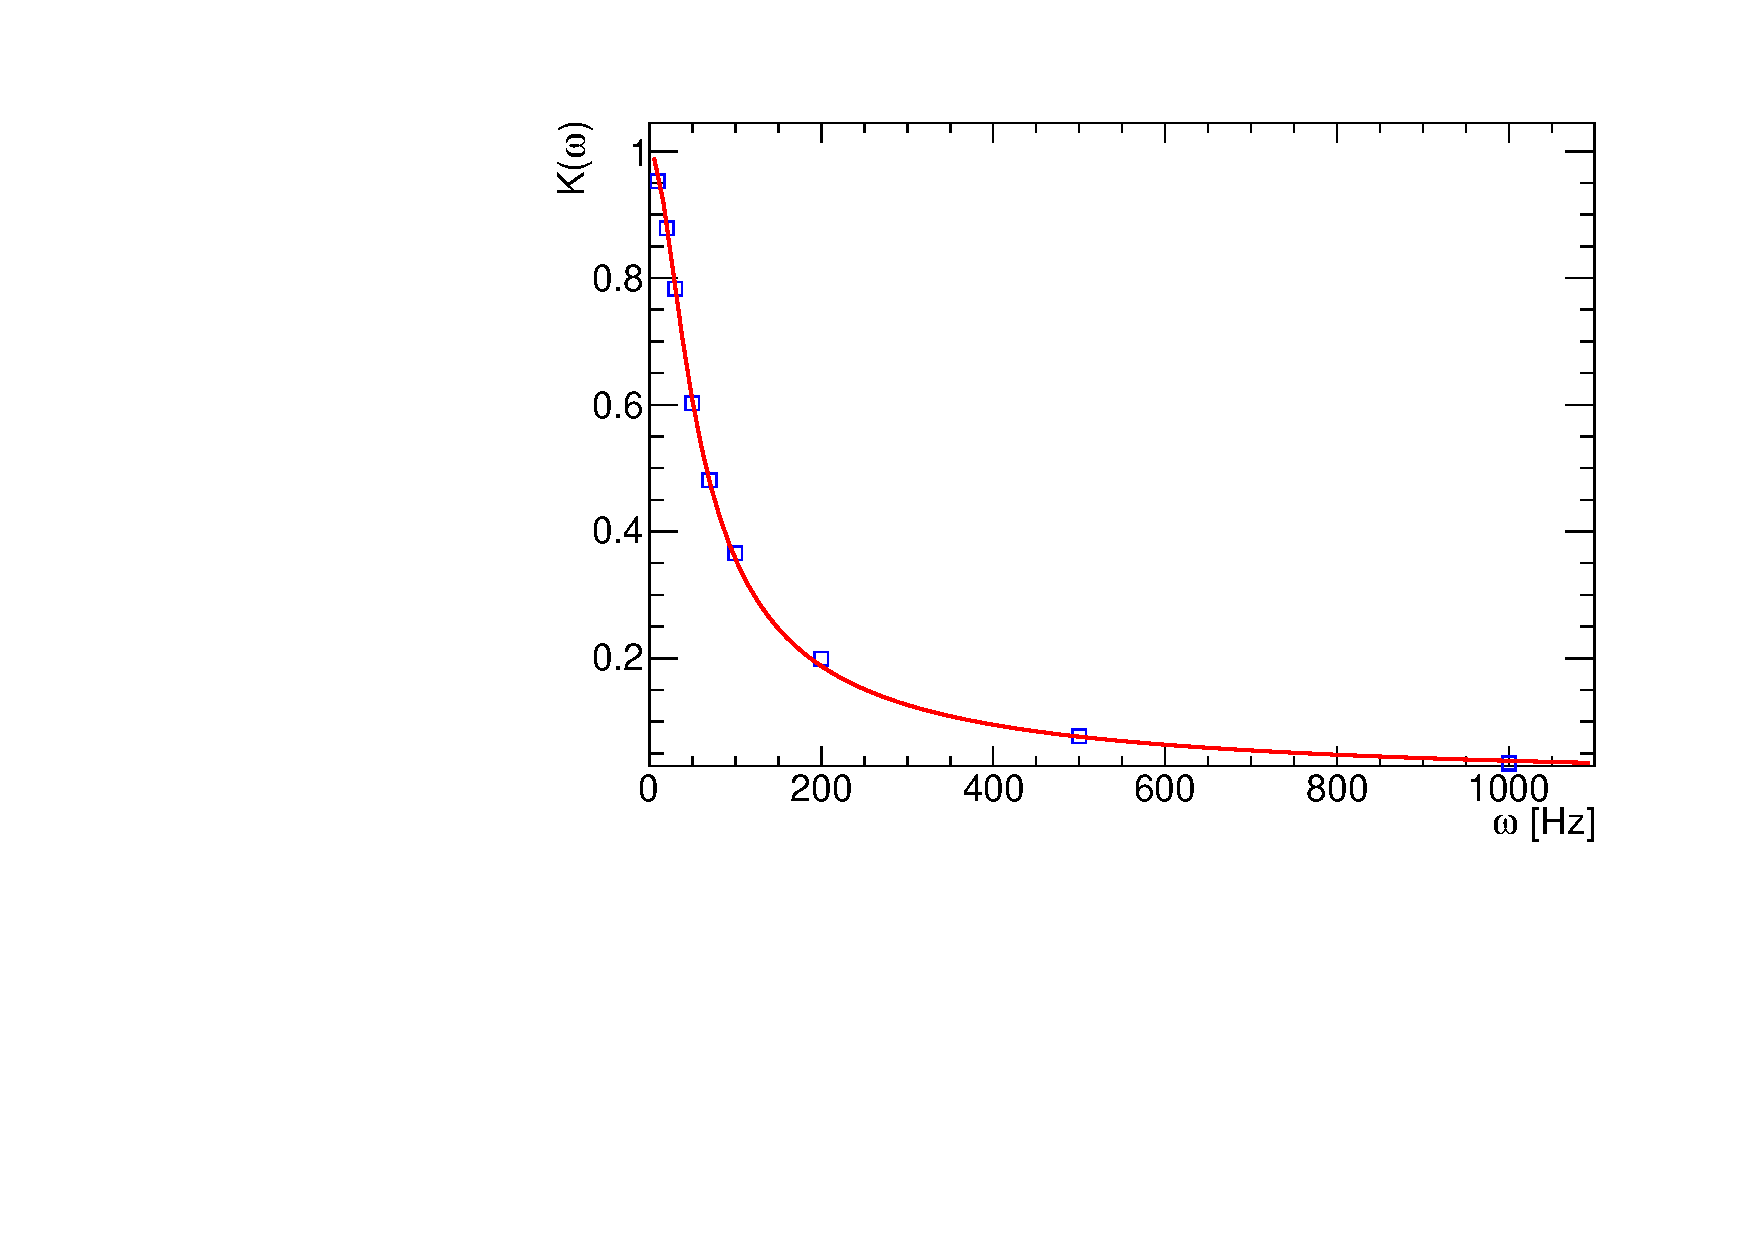
\includegraphics[width=1\linewidth]{sini/k.pdf}} \\$K(\omega)$ для інтегруючого чотирьохполюсника
	\end{minipage}
	\hfill
	\begin{minipage}[h]{0.47\linewidth}
		\center{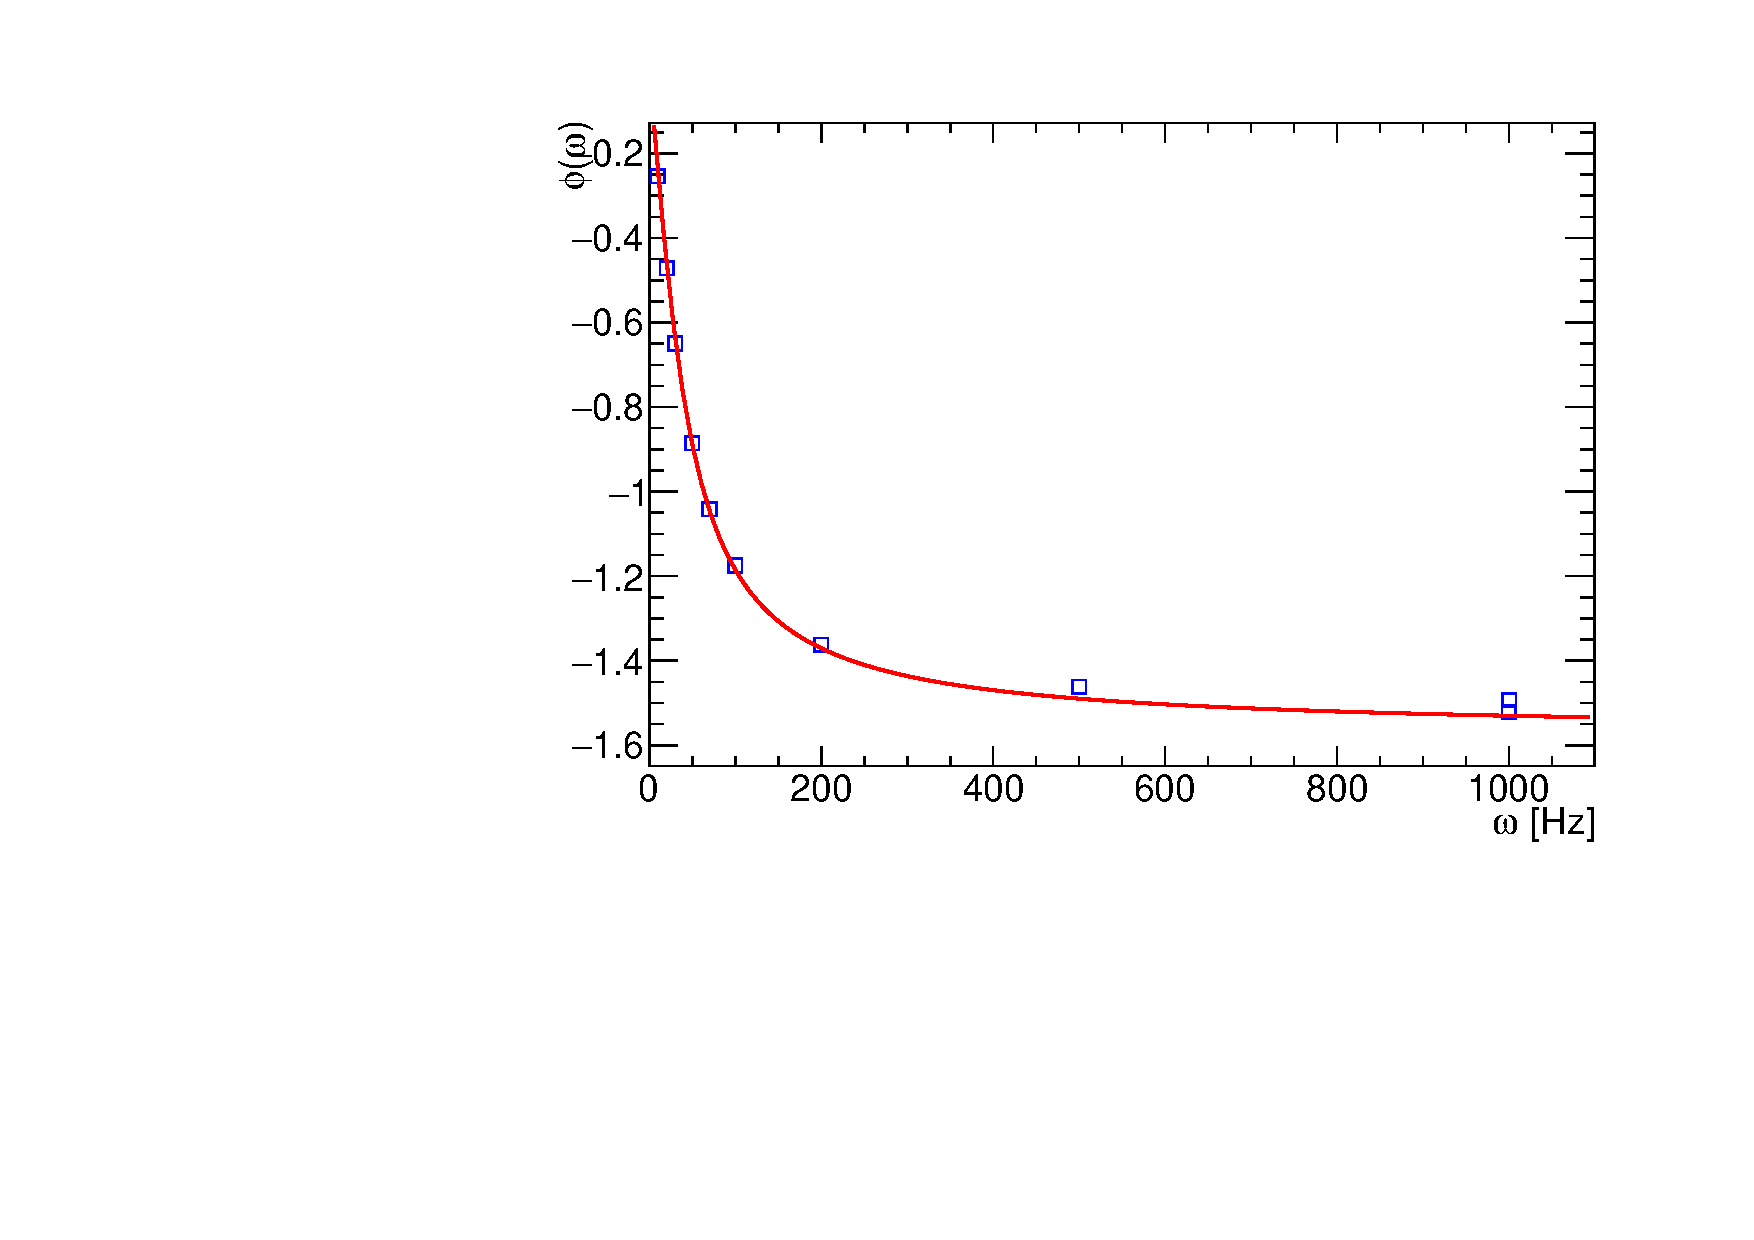
\includegraphics[width=1\linewidth]{sini/phi.pdf}} \\$\phi(\omega)$ для інтегруючого чотирьохполюсника
	\end{minipage}
	\caption{Отримані залежності відношення амплітуд $K(\omega)$ та зсуву фаз $\phi(\omega)$. Було апроксимано відповідно до моделей \ref{theoryD} та \ref{theoryI}}
	\label{fig:expkph}
\end{figure}

% \subsection{Дифферинціююча конфігурація}

% На відміну від текстових процесорів, що працюють за принципом {WYSIWYG} (What You See Is What You Get~--- що бачиш, те і отримуєш), \LaTeX{}, не маючи графічного інтерфейсу, формує результуючий документ з текстового файлу, що містить окремо власне текст і окремо інструкцію з його форматування, в термінах \LaTeX{} --- преамбулу.

% Текст документу може розбиватися на декілька окремих файлів для полегшення роботи над частинами документу або розподілення її між кількома людьми. Крім того, в окремі файли виносяться бібліографічні посилання у форматі BibTeX та рисунки, що включаються до документу. 

% Після завершення роботи над документом і запуском \LaTeX{}, він підключає вказані у преамбулі пакети макросів та опрацьовує файли проекту один, а за необхідності~--- декілька разів послідовно. При цьому, ним та супутніми програмами, такими як BibTeX, послідовно формуються тимчасові файли, що містять, наприклад, список бібліографії, посилань та змісту, а після~--- dvi (device indenendant) файл. Остайній придатний для перегляду та друку на будь"=якому комп'ютері з встановленим відповідним для нього dvi"=драйвером. При цьому гарантується однаковість форматування тексту на будь"=якому комп'ютері \cite[с.~16]{Lvovskii2010NaborVerstka}.

% За необхідності, dvi"=файл може бути конвертований до інших форматів, серед яких~--- широко розповсюджений pdf \cite{Habr2012BacDiplom}\cite{Habr2012TempDisser}.

% \subsection{Використання макророзширень в \LaTeX{}}

% Основною частиною системи LaTeX є велика кількість пакетів макросів, кожен з яких забезпечує автоматизацію і полегшення виконання тих чи інших дій при створенні документу або вносить зміни в стандартні налаштування \LaTeX{}. На момент написання статті офіційний веб-ресурс LaTeX~\cite{www:ctan} пропонує 5287 пакетів макросів. 

% Макрос представляє собою команду з назвою, що визначається або перевизначається наступними командами\cite{Sjutkin2002Manual}:
% \begin{verbatim}
% \newcommand{<назва команди>}[<кількісь параметрів>]{<тіло команди>}
% \renewcommand{<назва команди>}[<кількісь параметрів>]{<тіло команди>}
% \end{verbatim}

% Назви всіх команд у \LaTeX{} починаються з символу зворотнього слешу <<$\backslash$>>. Кількість параметрів не може перевищувати 9. Для подолання обмеження можуть використовуватися пакети, наприклад, обраний xkeyval (таблиця \ref{table:packages}), що створюють власний механізм передачі аргументів в макрос. В тілі макросу отримані аргументи використовуються за своїм номером за порядком після символу <<\# >>.

% Приклад простого макросу, що додає до документа перший параметр напівжирним а другий~--- курсивним шрифтом:
% \begin{verbatim}
% \newcommand{\boldAndItalik}[2]{\textbf{#1} \textit{#2}}
% \end{verbatim}

% Можливе використання попереднього макросу. На рисунку \ref{ris:image} зображено результат його роботи (збільшено).
% \begin{verbatim}
% \boldAndItalik{FirstText}{SecondText}
% \end{verbatim}


% \begin{figure}[ht]
% \center{
\includegraphics[width=1\linewidth]{img/makrosResultImg}}
% \caption{Зразок роботи макросу}
% \label{ris:image}
% \end{figure}

% Так як частина з існуючих пакетів макросів надає різні інструменти для реалізації одних і тих самих елементів, то було поставлено завдання обрати серед них необхідні для реалізації всіх поставлених задач з реалізації шаблону. Основні пакети, підключені до шаблону, перечислено в таблиці \ref{table:packages}

% \begin{table}{|l|l|}{Основні підключені пакети}{table:packages}
% 	{\hline
% 	\parbox[t]{5cm}{Назва} & Опис \\
% 	\hline}
% 	fontenc & Дозволяє вказати кодування документа\\
% 	cmap & Забезпечує коректне кодування\\
% 	babel & Забезпечує необхідні мовні зміни\\
% 	geometry & Дозволяє змінити параметри сторінки\\
% 	indentfirst & Забезпечує відступ у першому абзаці\\
% 	hyperref & Позначає деякі елементі як гіперпосилання\\
% 	fancyhdr & Дозволяє налаштувати колонтитули\\
% 	titlesec & Дозволяє налаштувати вигляд заголовків\\
% 	titletoc & Дозволяє налаштувати вигляд змісту\\
% 	longtable & Надає потужніші таблиці і налаштування для них\\
% 	caption & Дозволяє налаштувати підписи різних елементів\\
% 	xkeyval & Надає новий спосіб передачі параметрів у макрос\\
% 	ifthen & Надає макрос\,--\,умовний оператор\\
% \end{table}

% При цьому, зроблений вибір ніяк не обмежує користувачів шаблону у підключенні інших, альтернативних або власних пакетів.

% \subsection{Базові види документів}

% Кожен документ в \LaTeX{} належить до одного з видів, <<класів>> в термінах \LaTeX{}, стандартних, що йдуть з самим \LaTeX{} або тих, що привносяться пакетами. В таблиці \ref{table:classes} наведено основні класи документів.

% \begin{table}{|l|l|}{Основні вбудовані класи документів \LaTeX{}}{table:classes}
% 	{\hline
% 	\parbox[t]{5cm}{Назва} & Опис \\
% 	\hline}
% 	article & Статті для журналів, короткі звіти\\
% 	report & Великі звіти з кількох частин\\
% 	exreport & оновлений і розширений report\\
% 	book & Книга\\
% 	letter & Лист\\
% 	beamer & Презентація\\
% \end{table}

% Всі інші класи документів, що входять до складу пакетів або розроблюються автором самостійно для власних потреб, засновуються на одному з базових класів і зберігаються в окремому файлі з розширенням cls і іменем\,--\,назвою класу. Користувацькі класи підключаються до документу і працюють аналогічно базовим. 

% \section{Основні можливості \LaTeX{}}

% \subsection{Рубрикація документу}

% Відповідно до вимог \cite{DSTU20153008}, документ розбивається на структурні частини, серед яких <<Вступ>>, <<Зміст>>, <<Висновки>>, <<Список використаних джерел>>, <<Додатки>> та, власне, текст документу, який теж розбивається на менші частини~--- розділи, підрозділи, пункти та підпункти. \LaTeX{} надає механізми для форматування заголовків всіх цих частин, проте їхнє овормлення не сповна відповідає накладеним вимогам. Їх опис та необхідні зміни описані в \ref{dev:toc}.

% Зміст, як і деякі інші структурні частини документу, формується засобами \LaTeX{} автоматично з заголовків згідно вказаних налаштувань і заданого форматування. Детальніше внесені зміни розглянуто в \ref{dev:toc}.

% Текстові процесори, найпопулярнішими серед яких є MS Word та OO Writer, надають досить потужні засоби для форматування та структурного розділення документу у вигляді стилів. Проте, все ще широко розповсюджене некоректне використання засобів текстових процесорів, призводить до того, що форматування до кожного елементу тексту авторами застосовується вручну. Це, як і стиль набору, який подекуди називають <<вирівнювання пробілами>>, дає в результаті документи низької якості, які складно піддаються відносно простим змінам. 

% На рисунку \ref{ris:wrongFormat} наведено декілька типових помилок форматування: <<вирівнювання пробілами>> на титульному аркуші (a); <<зміст>>, сформований вручну, в якому, крім зайвих пробілів, присутнє порушення вимог до оформлення (c); заголовки, не сповна коректно оформлені, та абзацний відступ з пробілів; формула та її номер, вирівняні пробілами. 

% \begin{figure}[h]
% 	\begin{minipage}[h]{0.47\linewidth}
% 		\center{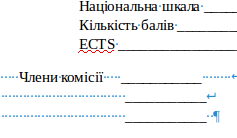
\includegraphics[width=1\linewidth]{img/wrongFormatA}} a) \\
% 	\end{minipage}
% 	\hfill
% 	\begin{minipage}[h]{0.47\linewidth}
% 		\center{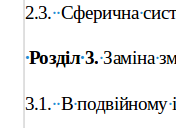
\includegraphics[width=1\linewidth]{img/wrongFormatB}} \\b)
% 	\end{minipage}
% 	\vfill
% 	\begin{minipage}[h]{0.47\linewidth}
% 		\center{
\includegraphics[width=1\linewidth]{img/wrongFormatC}} c) \\
% 	\end{minipage}
% 	\hfill
% 	\begin{minipage}[h]{0.47\linewidth}
% 		\center{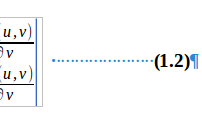
\includegraphics[width=1\linewidth]{img/wrongFormatD}} d) \\
% 	\end{minipage}
% 	\caption{Некоректне форматування документу в текстовому процесорі}
% 	\label{ris:wrongFormat}
% \end{figure}

% \LaTeX{} не дозволить використовувати прийоми, подібні наведеним на рисунку \ref{ris:wrongFormat}, для форматування тексту, що змусить автора користуватись коректними засобами форматування та, цим самим, підвищить якість готового до друку або перегляду документу.

% \subsection{Ведення бібліографії}

% Бібліографічні посилання в структурній частині <<Список використаних джерел>> мають наводитися відповідно до ДСТУ 7.1. Автоматична нумерація посилань і їх формування суттєво спрощують роботу над документом. 

% Для роботи з бібліографічними посиланнями використовується BibTeX. Опрацьовуючи тимчасовий файл з посиланнями та текстовий файл з бібліографічними посиланнями у власному форматі, ним формується список використаної літератури, впорядкований за порядком першого входження цитат. Цей файл використовується \LaTeX{} при наступному опрацюванні документу.

% Саме через те, що деякі зміни вносяться в тимчасові файли вже після опрацювання частини тексту, для отримання коректного документу (коректного за змістом, нумерацією бібліографії та посилань а не власне форматуванням) необхідно запускати \LaTeX{} декілька разів  (до чотирьх \cite{Stolyarov2010SverstaiDiplom}) поспіль.

% \subsection{Автоматизовані процеси}

% Пакет дозволяє автоматизувати значну кількість задач по підготовці наукових статей, серед яких вже згадані вище формування змісту; нумерація заголовків всіх рівнів, формул, таблиць та ілюстрацій; розміщення ілюстрацій і таблиць на аркуші; ведення бібліографії тощо.
